\documentclass[compress,red]{beamer}
\usepackage{etex}
\mode<presentation>

\usetheme{Warsaw}
%\usetheme{Madrid}

\setbeamertemplate{navigation symbols}{}
\setbeamertemplate{headline}{}

\setbeameroption{show notes}
%\setbeameroption{hide notes}

%\hypersetup{pdfpagemode=FullScreen} % makes your presentation go automatically to full screen
%\useoutertheme[subsection=false]{smoothbars}
\useoutertheme{shadow}

% include packages
\usepackage{subfigure}
\usepackage{textcomp}
\usepackage{multicol}
\usepackage{amsmath}
\usepackage{epsfig}
\usepackage{graphicx}
\usepackage[all,knot]{xy}
\xyoption{arc}
\usepackage{url}
\usepackage{multimedia}
\usepackage{hyperref}
\usepackage{helvet}
\usepackage[polish,english]{babel}
\usepackage[utf8]{inputenc}
\usepackage{multirow}
\usepackage{verbatim}
%\usepackage{geometry}
%\geometry{verbose,letterpaper}
%\usepackage{movie15}
%\usepackage{hyperref}
\usepackage{pgfpages}


%\logo{}
\titlegraphic{\scalebox{4}{
    
\includegraphics[height=0.5cm]{../pictures/ohwr_logo.eps}
  }
}


%\title{F*WATCH, making a watch differently!}
\title[{\makebox[.45\paperwidth]{F*WATCH\hfill%
       \insertframenumber/\inserttotalframenumber}}]{F*WATCH, making a watch differently!}


\author % (optional, use only with lots of authors)
{Federico Vaga, Matthieu Cattin}
% - Give the names in the same order as the appear in the paper.
% - Use the \inst{?} command only if the authors have different
%   affiliation.

%\institute%[Universities of Somewhere and Elsewhere] % (optional, but mostly needed)
%{
  %\inst{1}%
  %BE-CO Hardware and Timing section\\
  %CERN, Geneva, Switzerland
 %\and
 %\inst{2}%
 %Department of Theoretical Philosophy\\
 %University of Elsewhere
% }
% - Use the \inst command only if there are several affiliations.
% - Keep it simple, no one is interested in your street address.

\date %(optional, should be abbreviation of conference name)
{FOSDEM, Brussels, 31 January 2015}
% - Either use conference name or its abbreviation.
% - Not really informative to the audience, more for people (including
%   yourself) who are reading the slides online

%\subject{Theoretical Computer Science}
% This is only inserted into the PDF information catalog. Can be left
% out.


% If you have a file called "university-logo-filename.xxx", where xxx
% is a graphic format that can be processed by latex or pdflatex,
% resp., then you can add a logo as follows:

%\pgfdeclareimage[height=1cm]{ohr-logo}{ohr_logo.jpg}
%\logo{\pgfuseimage{ohr-logo}}


% Delete this, if you do not want the table of contents to pop up at
% the beginning of each subsection:
%\AtBeginSection[]
%{
%  \begin{frame}<beamer>{Outline}
%    \tableofcontents[currentsection]
%  \end{frame}
%}


% If you wish to uncover everything in a step-wise fashion, uncomment
% the following command:

%\beamerdefaultoverlayspecification{<+->}


\begin{document}

\begin{frame}
  \titlepage
  \note[item]{Introduce speakers.}
  \note[item]{We're going to talk about a after-work project we made last summer with a few other colleagues from CERN.}
\end{frame}

%\begin{frame}{Outline}
%  \tableofcontents
  % You might wish to add the option [pausesections]
%\end{frame}


% Structuring a talk is a difficult task and the following structure
% may not be suitable. Here are some rules that apply for this
% solution:

% - Exactly two or three sections (other than the summary).
% - At *most* three subsections per section.
% - Talk about 30s to 2min per frame. So there should be between about
%   15 and 30 frames, all told.

% - A conference audience is likely to know very little of what you
%   are going to talk about. So *simplify*!
% - In a 20min talk, getting the main ideas across is hard
%   enough. Leave out details, even if it means being less precise than
%   you think necessary.
% - If you omit details that are vital to the proof/implementation,
%   just say so once. Everybody will be happy with that.



%#####################################################################
%############ SECTION ################################################
\section{Introduction}

\subsection*{} % dummy subsection to display dots

%------------ FRAME --------------------------------------------------
\begin{frame}{Why making another watch?}

  \begin{block}{Gift}
    \begin{itemize}
%    \item 
    \item for a retiring colleague
    \end{itemize}
  \end{block}

\end{frame}

%------------ FRAME --------------------------------------------------
\begin{frame}{What is it?}


\end{frame}


%#####################################################################
%############ SECTION ################################################
\section{The design}

\subsection*{} % dummy subsection to display dots

%------------ FRAME --------------------------------------------------
\begin{frame}{Features}

  \begin{block}{}
    \begin{itemize}
    \item Low power MCU
    \item LCD display (+ backlight)
    \item micro-USB connector (charging, data transfer)
    \item Li-ion battery (+ fuel gauge)
    \item microSD card
    \item 4 buttons
    \item GPS module
    \item Pressure sensor (altitude, barometer)
    \item Compass
    \item 3D accelerometer
    \item Ambient light sensor (backlight adjustment)
    \item Buzzer
    \item Vibrating motor
    \end{itemize}
  \end{block}

  \note[item]{}

\end{frame}

%------------ FRAME --------------------------------------------------
\begin{frame}{Component selection}

  \begin{block}{Criteria}
    \begin{itemize}
    \item Low power consumption
    \item Available from main suppliers
    \item Small footprint
    \item ...
    \end{itemize}
  \end{block}

  \note[item]{}

\end{frame}

%------------ FRAME --------------------------------------------------
\begin{frame}{GPS module}

  \begin{block}{M10478-A1}
    \begin{itemize}
    \item Antenova
    \item 13 x 9.5 x 1.8mm
    \item Integrated antenna
    \end{itemize}
  \end{block}

  \begin{center}
    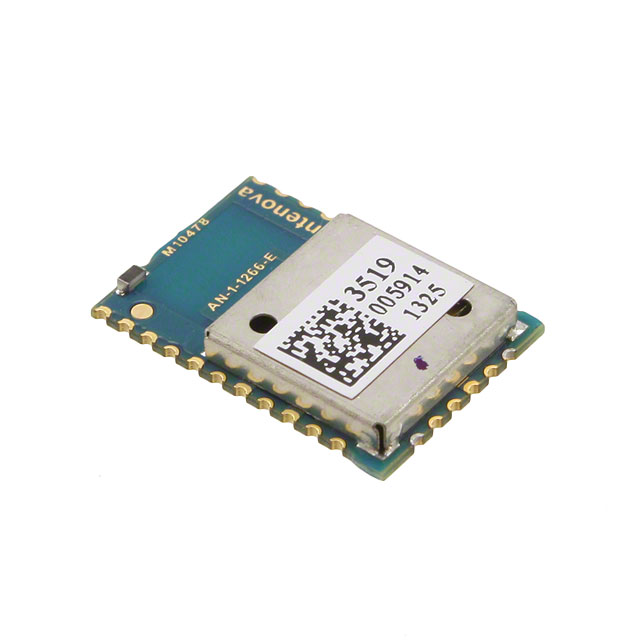
\includegraphics[height=5cm]{../pictures/M10478-A1.eps}
  \end{center}

  \note[item]{}

\end{frame}

%------------ FRAME --------------------------------------------------
\begin{frame}{Altimeter module (pressure sensor)}

  \begin{block}{MS5806-02BA}
    \begin{itemize}
    \item Measurement Specialties
    \item 6.4 x 4 x 2.8mm
    \item Water resistant
    \end{itemize}
  \end{block}

  \begin{center}
    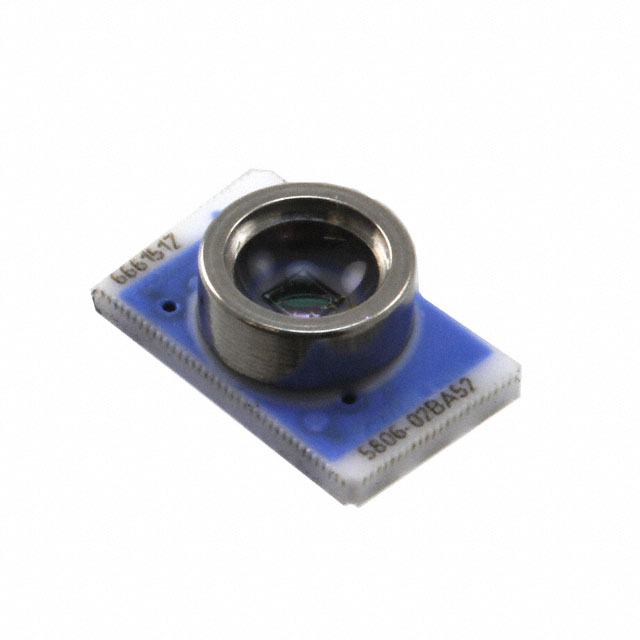
\includegraphics[height=4.5cm]{../pictures/MS5806-02BA52-51.eps}
  \end{center}

  \note[item]{}

\end{frame}

%------------ FRAME --------------------------------------------------
\begin{frame}{Display}

  \begin{block}{Memory LCD}
    \begin{itemize}
    \item Sharp
    \item 128 x 128 pixels (1.28 inches)
    \item Ultra low current
    \end{itemize}
  \end{block}


  \begin{center}
    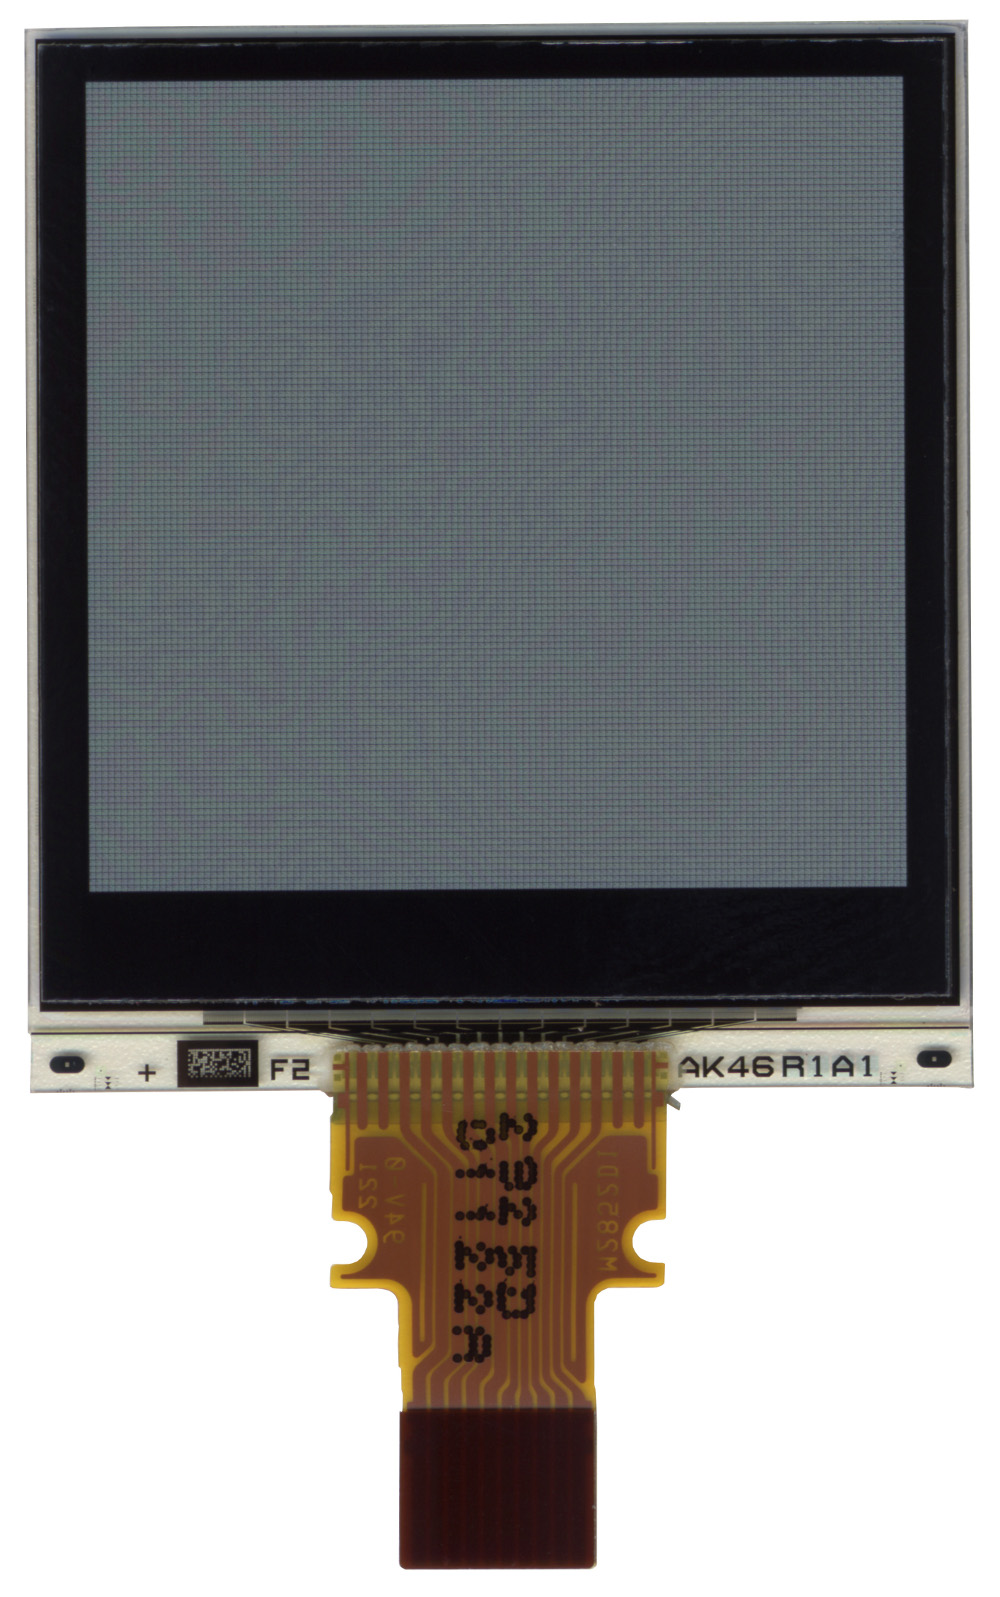
\includegraphics[height=4.5cm]{../pictures/LCD.eps}
  \end{center}

  \note[item]{}

\end{frame}

%------------ FRAME --------------------------------------------------
\begin{frame}{Battery}

  \begin{block}{}
    \begin{itemize}
    \item Adafruit
    \item Li-ion 500mAh
    \item Lightweight, big capacity
    \end{itemize}
  \end{block}

  \begin{center}
    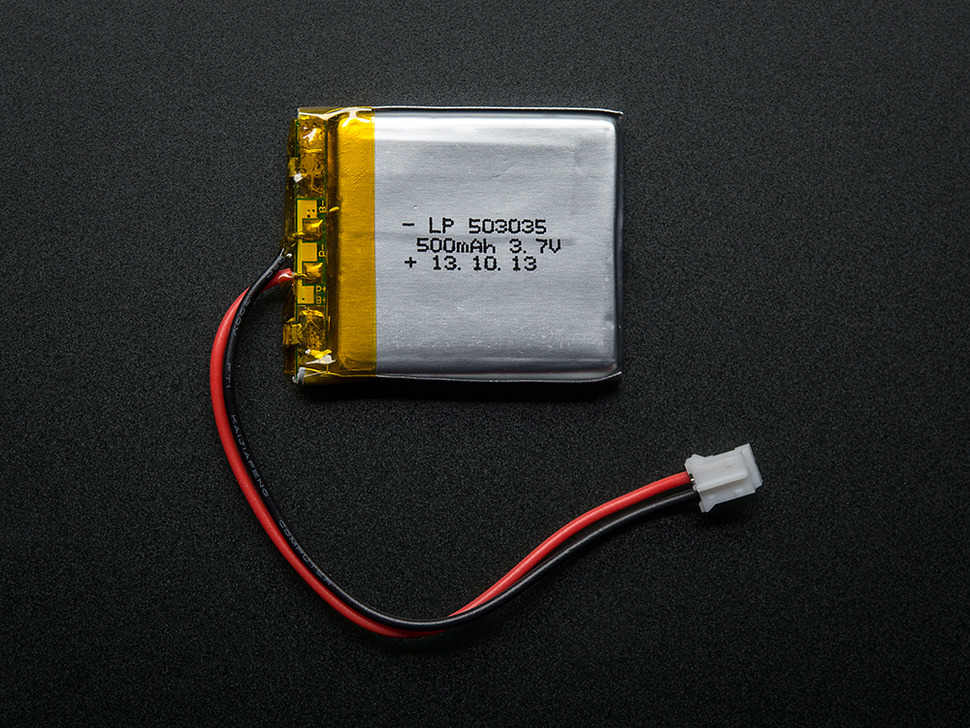
\includegraphics[height=5cm]{../pictures/battery.eps}
  \end{center}

  \note[item]{}

\end{frame}

%------------ FRAME --------------------------------------------------
\begin{frame}{PCB design}

  \begin{block}{EDA tool choice}
    \begin{itemize}
    \item KiCad
    \item CERN is contributing
    \item Developer next door (help, bugfix, feedback)
    \item 
    \end{itemize}
  \end{block}

  \begin{center}
    
\includegraphics[height=1cm]{../pictures/kicad_logo.eps}
  \end{center}

  \note[item]{}

\end{frame}

%------------ FRAME --------------------------------------------------
\begin{frame}{PCB design}

  \begin{block}{Characteristics}
    \begin{itemize}
    \item 4 x 4 cm
    \item 4 layers
    \item Components on both sides
    \item Manufactered by Eurocircuits
    \end{itemize}
  \end{block}

  \begin{center}
    %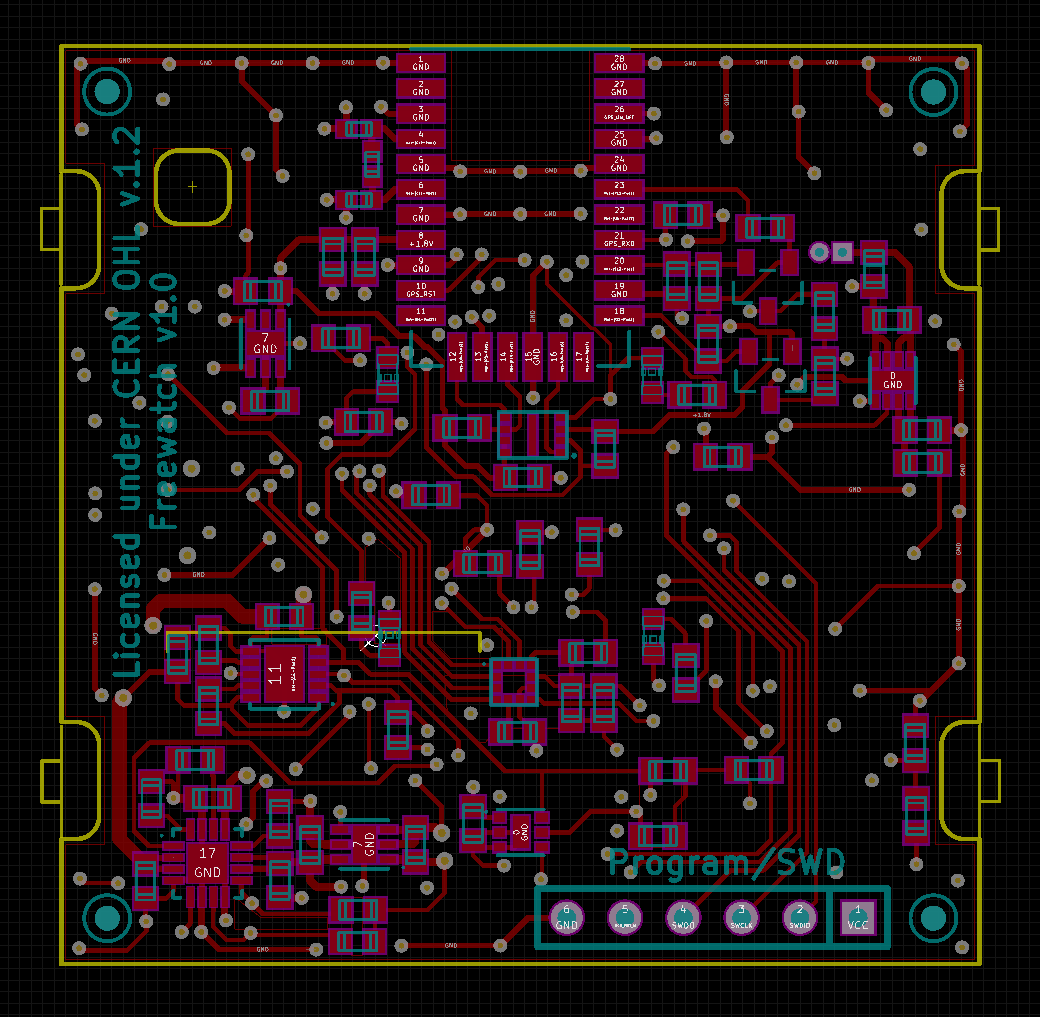
\includegraphics[height=1cm]{../pictures/pcb_top.eps}~
    %\includegraphics[height=1cm]{../pictures/pcb_bot.eps}
  \end{center}

  \note[item]{}

\end{frame}

%------------ FRAME --------------------------------------------------
\begin{frame}{PCB assembly}

  \begin{block}{}
    \begin{itemize}
    \item Stencils (ordered with PCB)
    \item Leaded soldering paste (easier to handle than lead-free)
    \item Components placed by hand (script to generate placement pdf)
    \item Soldered with hot-air station (quite tricky!)
    \end{itemize}
  \end{block}

  \begin{center}
    %\includegraphics[height=1cm]{../pictures/pcb_assembly.eps}
    %\includegraphics[height=1cm]{../pictures/placement_pdf.eps}
  \end{center}

  \note[item]{}

\end{frame}

%------------ FRAME --------------------------------------------------
\begin{frame}{PCB test}

  \begin{block}{First prototype fully working, except...}
    \begin{itemize}
    \item ... one error in a footprint (voltage regulator)
    \item ... MCU interrupt scheme
      \begin{itemize}
      \item Polling for charger state
      \item Draining the battery quickly
      \item Fixed with few wires!
      \end{itemize}
    \end{itemize}
  \end{block}

  \begin{center}
    %\includegraphics[height=1cm]{../pictures/pcb_assembly.eps}
  \end{center}

  \note[item]{}

\end{frame}

%------------ FRAME --------------------------------------------------
\begin{frame}{Mechanical design}

  \begin{block}{CAD tool selection}
    \begin{itemize}
    \item No mechanical designer in the team
    \item Evaluate existing free CAD tools (Freecad, ...)
    \item Docmentation, support
    \item Leanring curve, user-friendliness
    \end{itemize}
  \end{block}

  \begin{itemize}
  \item Decided to use \textbf{Freecad}
  \end{itemize}

  \begin{center}
    
\includegraphics[height=2cm]{../pictures/freecad_logo.eps}
  \end{center}

\end{frame}

%------------ FRAME --------------------------------------------------
\begin{frame}{Mechanical design}

  \begin{block}{Challenges}
    \begin{itemize}
    \item Learn Freecad
    \item Buttons
    \item Water-resistance (dropped for proto)
    \item Size
    \item Wrist-strap
    \item 3D printing (new for us)
    \end{itemize}
  \end{block}

  \note[item]{Learn Freecad = show the making of video}
  \note[item]{Button = show detailed cut-view of button and explain quickly}
  \note[item]{Water-resistance = show, explain grove and rubber join idea}
  \note[item]{Size = keep it reasonably small to be wearable on the wrist}
  \note[item]{Wrist-strap = easy to get "nato" type wrist-strap, bought online}
  \note[item]{3D printing = didn't knew the domain, studied the main 3d printing services, }
  \note[item]{}

\end{frame}

%------------ FRAME --------------------------------------------------
\begin{frame}{3D model}

  \begin{center}
    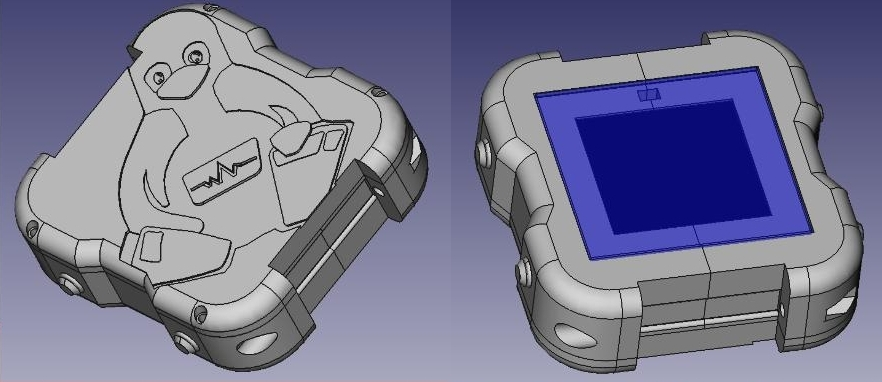
\includegraphics[height=4.8cm]{../pictures/case-design-model.eps}
  \end{center}

\end{frame}

%------------ FRAME --------------------------------------------------
\begin{frame}{First 3D print}

  \begin{itemize}
  \item Made of platic (powder)
  \end{itemize}

  \begin{center}
    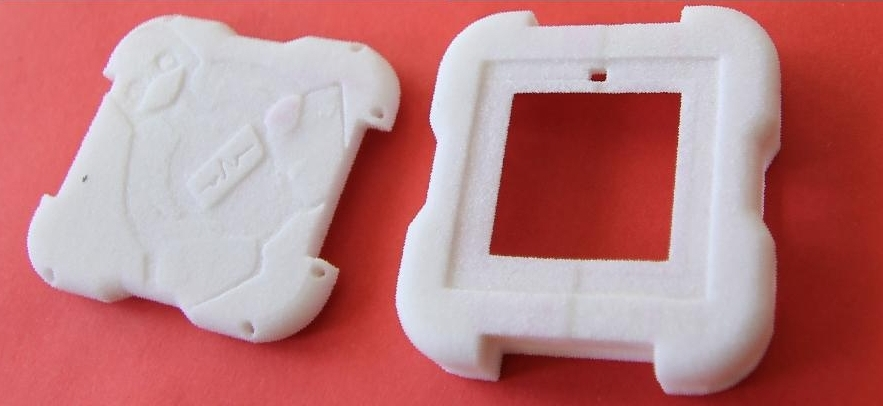
\includegraphics[height=5cm]{../pictures/case-design-print-v2.eps}
  \end{center}

\end{frame}

%------------ FRAME --------------------------------------------------
\begin{frame}{Second 3D print}

  \begin{itemize}
  \item Made of resin (liquid)
  \end{itemize}

  \begin{center}
    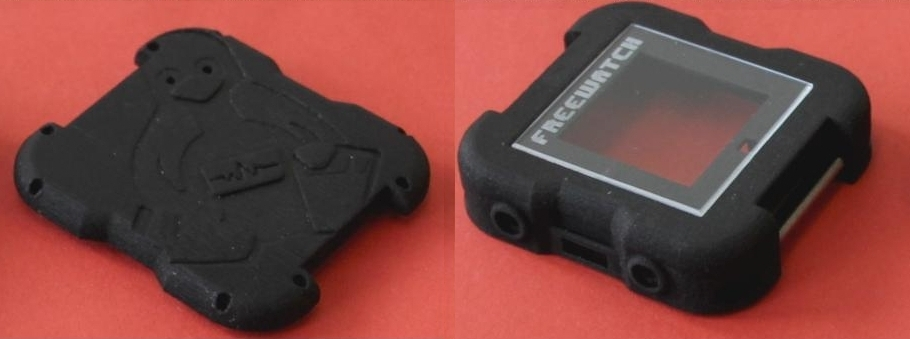
\includegraphics[height=4.1cm]{../pictures/case-design-print-v3.eps}
  \end{center}

\end{frame}

%------------ FRAME --------------------------------------------------
\begin{frame}{Software (firmware, host software)}

  \begin{center}
    %\includegraphics[height=7cm]{../pictures/spec_v4.eps}
  \end{center}

  \note[item]{}

\end{frame}


%#####################################################################
%############ SECTION ################################################
\section{The tools / the message}

\subsection*{} % dummy subsection to display dots

%------------ FRAME --------------------------------------------------
\begin{frame}{Mechanical design}


  \note[item]{}

\end{frame}

%------------ FRAME --------------------------------------------------
\begin{frame}{PCB design}

  \begin{center}
    %\includegraphics[height=6cm]{../pictures/spec-fmc-adc_arch_simple_color.eps}
  \end{center}

  \note[item]{}

\end{frame}

%------------ FRAME --------------------------------------------------
\begin{frame}{Software}

  \begin{center}
    %\includegraphics[height=6cm]{../pictures/spec-fmc-adc_arch_simple_color.eps}
  \end{center}

  \note[item]{}

\end{frame}


%#####################################################################
%############ SECTION ################################################
\section{Building a watch}

\subsection*{} % dummy subsection to display dots

%------------ FRAME --------------------------------------------------
\begin{frame}{I want to build this watch, what should I do?}

  \begin{block}{Tools and techniques}
    \begin{itemize}
    \item Soldering QFN/BGA (stencil, paste)
    \item Hot-air station or oven
    \item Milling maching (optionnal for plexiglass)
    \end{itemize}
  \end{block}

  \note[item]{}

\end{frame}

%------------ FRAME --------------------------------------------------
\begin{frame}{How much does it costs?}

  \begin{block}{Estimated cost for small series (without shipping)}

  \begin{table}[h]
    \begin{tabular}{l|r|r|r|l}
      \cline{2-4}
      & \multicolumn{3}{c|}{Number of watches}                                     &  \\ \cline{2-4}
      & \multicolumn{1}{c|}{1} & \multicolumn{1}{c|}{10} & \multicolumn{1}{c|}{50} &  \\ \cline{1-4}
      \multicolumn{1}{|l|}{Pcb + components}         & 166 \texteuro                & 87 \texteuro                  & 73 \texteuro                  &  \\ \cline{1-4}
      \multicolumn{1}{|l|}{Pcb assembly}             & -                      & 104 \texteuro                 & 59 \texteuro                  &  \\ \cline{1-4}
      \multicolumn{1}{|l|}{Case + buttons + screws}  & 67 \texteuro                 & 65 \texteuro                  & 60 \texteuro                  &  \\ \cline{1-4}
      \multicolumn{1}{|l|}{\textbf{TOTAL per watch}} & \textbf{233 \texteuro}       & \textbf{256 \texteuro}        & \textbf{193 \texteuro}        &  \\ \cline{1-4}
      \multicolumn{1}{|l|}{\textbf{TOTAL}}           & \textbf{233 \texteuro}       & \textbf{2'558 \texteuro}      & \textbf{9'630 \texteuro}      &  \\ \cline{1-4}
    \end{tabular}
  \end{table}

  \end{block}


  \note[item]{}

\end{frame}


%#####################################################################
%############ SECTION ################################################
\section{What's next?}

\subsection*{} % dummy subsection to display dots

%------------ FRAME --------------------------------------------------
\begin{frame}{What's next?}

  \begin{block}{Improvements}
    \begin{itemize}
    \item Bluetooth LE
    \item Water-resistance
    \item LCD backlight
    \item Reduce PCB/housing size
    \item 
    \end{itemize}
  \end{block}

  \begin{block}{Software}
    \begin{itemize}
    \item Firmware loader
    \item Data transfer (to/from SD card)
    \item Emulator
    \item Application "ecosystem"
    \end{itemize}
  \end{block}

  \note[item]{}

\end{frame}

%------------ FRAME --------------------------------------------------
\begin{frame}{What's next?}

  \begin{block}{Build a community}
    \begin{itemize}
    \item 
    \item 
    \end{itemize}
  \end{block}

  \note[item]{}

\end{frame}

%------------ FRAME --------------------------------------------------
\begin{frame}{What's next?}

  \begin{block}{Make a kit}
    \begin{itemize}
    \item Pre-assembled PCB option
    \item Customisable strap/housing color
    \item Alternative housing
    \item Sold by a company?
    \end{itemize}
  \end{block}

  \note[item]{}

\end{frame}



%------------ FRAME --------------------------------------------------
\begin{frame}{Conclusions}

  \begin{block}{}
    \begin{itemize}
    \item 
    \item 
    \item 
    \item 
    \item 
    \end{itemize}
  \end{block}

  \note[item]{}

\end{frame}


\begin{comment}
\end{comment}


\end{document}


